\colorlet{outlinecolor}{brightpurple}

\colorlet{headercolor}{outlinecolor}
\colorlet{rowcolor1}{outlinecolor!70}
\colorlet{rowcolor2}{outlinecolor!50}

\begin{tikzpicture}
	\node [mybox, fill=boxcolor, draw=outlinecolor] (box){%
		\begin{minipage}{0.3\textwidth}
			\vspace{0.1cm}
			
			\underline{Introduction}: It's a best practice to create all your changes on \textcolor{outlinecolor}{feature (or topic) branches}, make sure these changes stable, and then merge into the \inlinebash{main} branch.
			
			\vspace{-2mm}
			\begin{center}
				\textcolor{background}{
					\begin{tabularx}{\textwidth}{>{\columncolor{rowcolor1}}X|>{\columncolor{rowcolor2}}p{3.5cm}}
						\arrayrulecolor{boxcolor} % Table line color
						\rowcolor{headercolor} % Header row color
						\multicolumn{1}{c|}{\centering \textbf{Git Command}} & \multicolumn{1}{c}{\centering \textbf{Description}} \\ % Center the header text
						\hline % Add a horizontal line below the header row
						\rowcolor{rowcolor1} % New Row
						\tablebash{git branch} & Lists all current \textbf{local} branches \\
						\rowcolor{rowcolor2} 
						\tablebash{git branch --all} & Lists all current local and remote branches \\
						\rowcolor{rowcolor1} 
						\tablebash{git branch -m old\_branch\_name new\_branch\_name} & Rename your Git branch \\
						\rowcolor{rowcolor2} 
						\tablebash{git branch --delete branch\_name} & Deletes a \textbf{local} branch\\
					\end{tabularx}
				}
			\end{center}
			\vspace{-1mm}
			
			\underline{Merging}: Insert the changes from one branch into another as a new commit. Main types of merges are:
			\begin{itemize}
				\item A \textcolor{outlinecolor}{fast forward merge} happens when one branch is ahead of another. i.e., \\
			\end{itemize}
			\hfill
			\begin{minipage}{0.45\textwidth} 
				\centering
				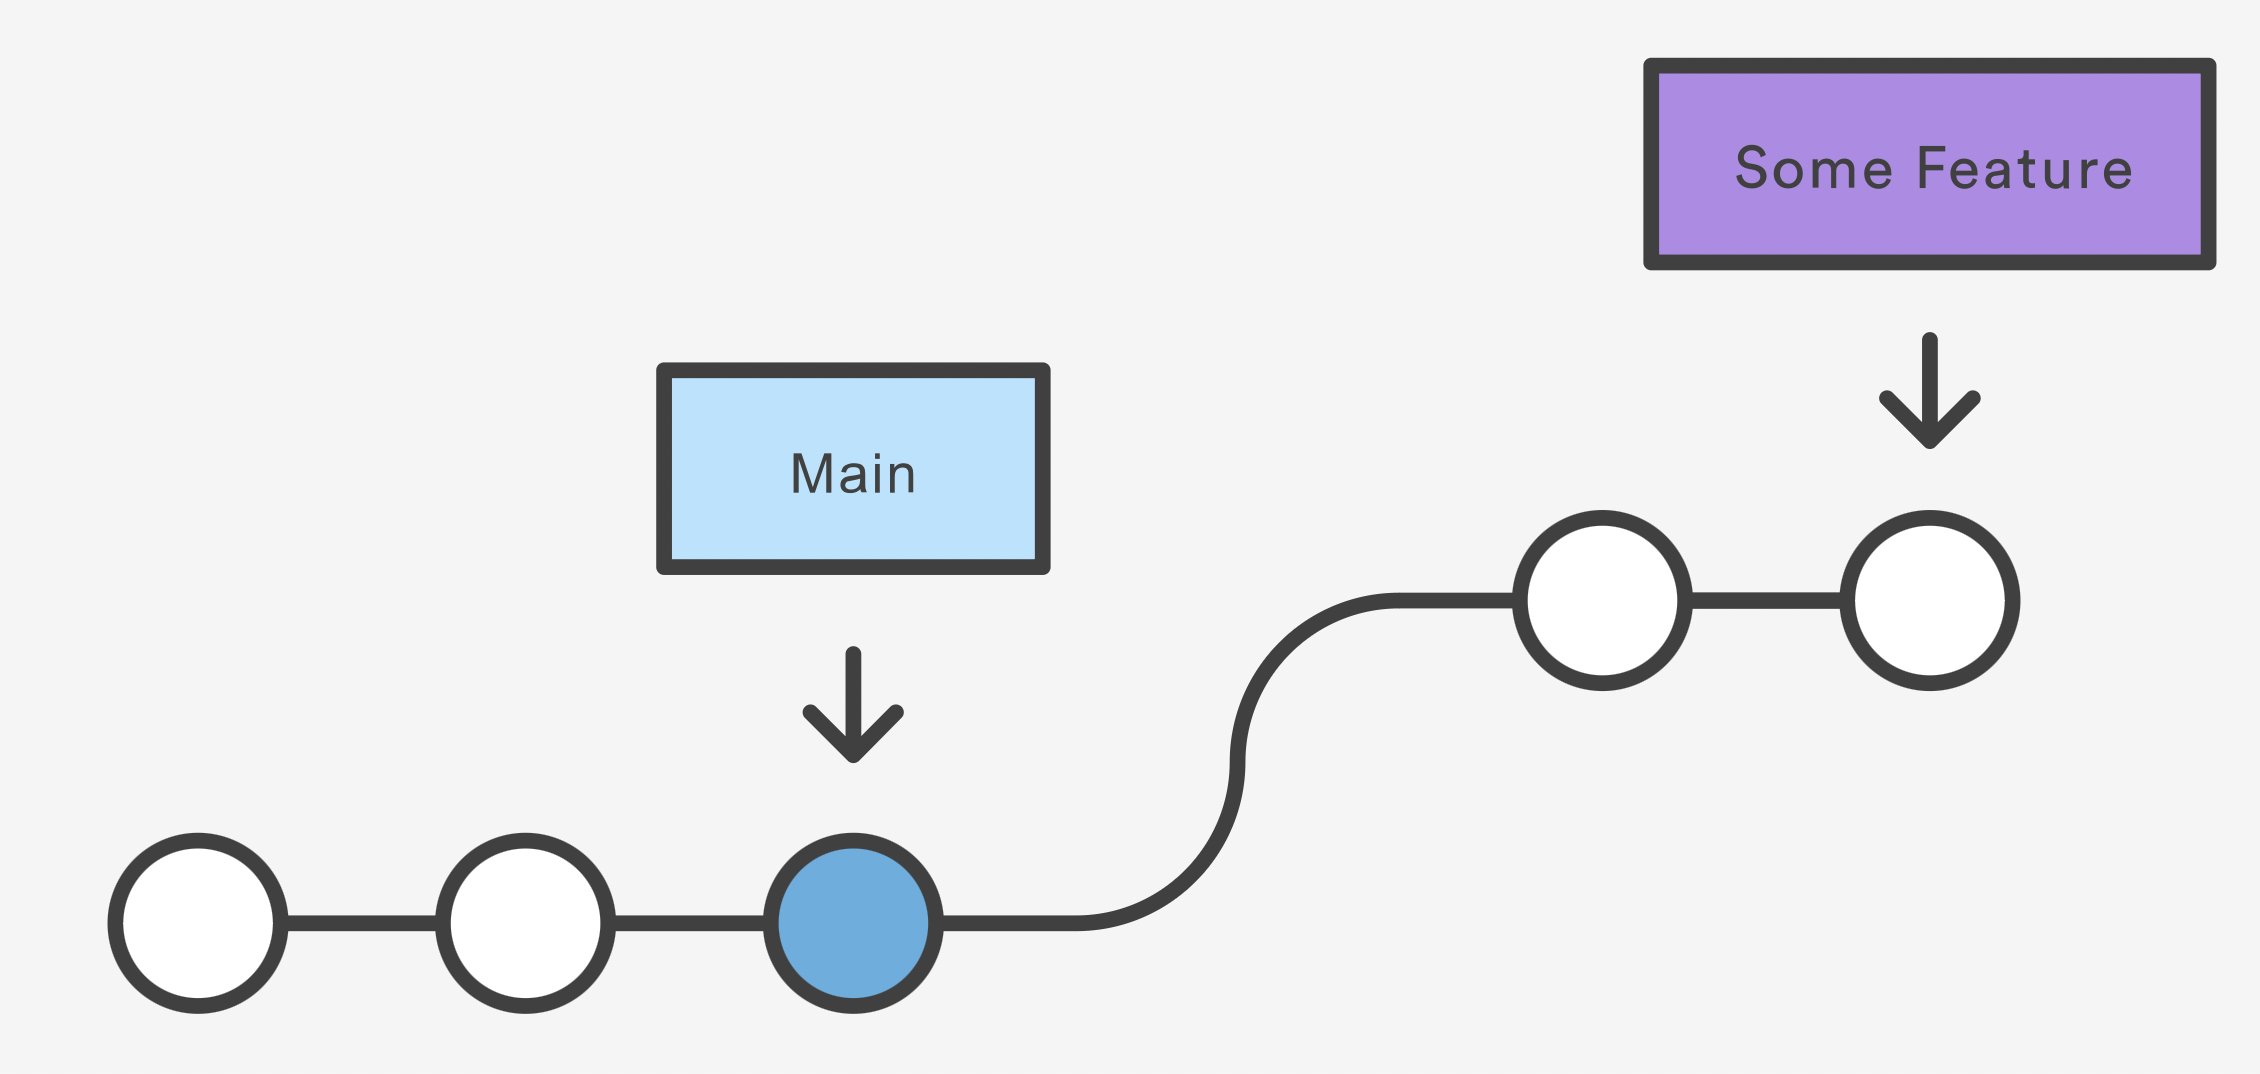
\includegraphics[width=\textwidth]{images/fast_forward_merge_before.png}
				\captionsetup{justification=centering}
				\captionof{figure}{Before a fast-forward merge. \href{https://www.atlassian.com/git/tutorials/using-branches/git-merge}{\faLink{} Source}}
			\end{minipage}%
			\hfill
			\begin{minipage}{0.4\textwidth}
				\centering
				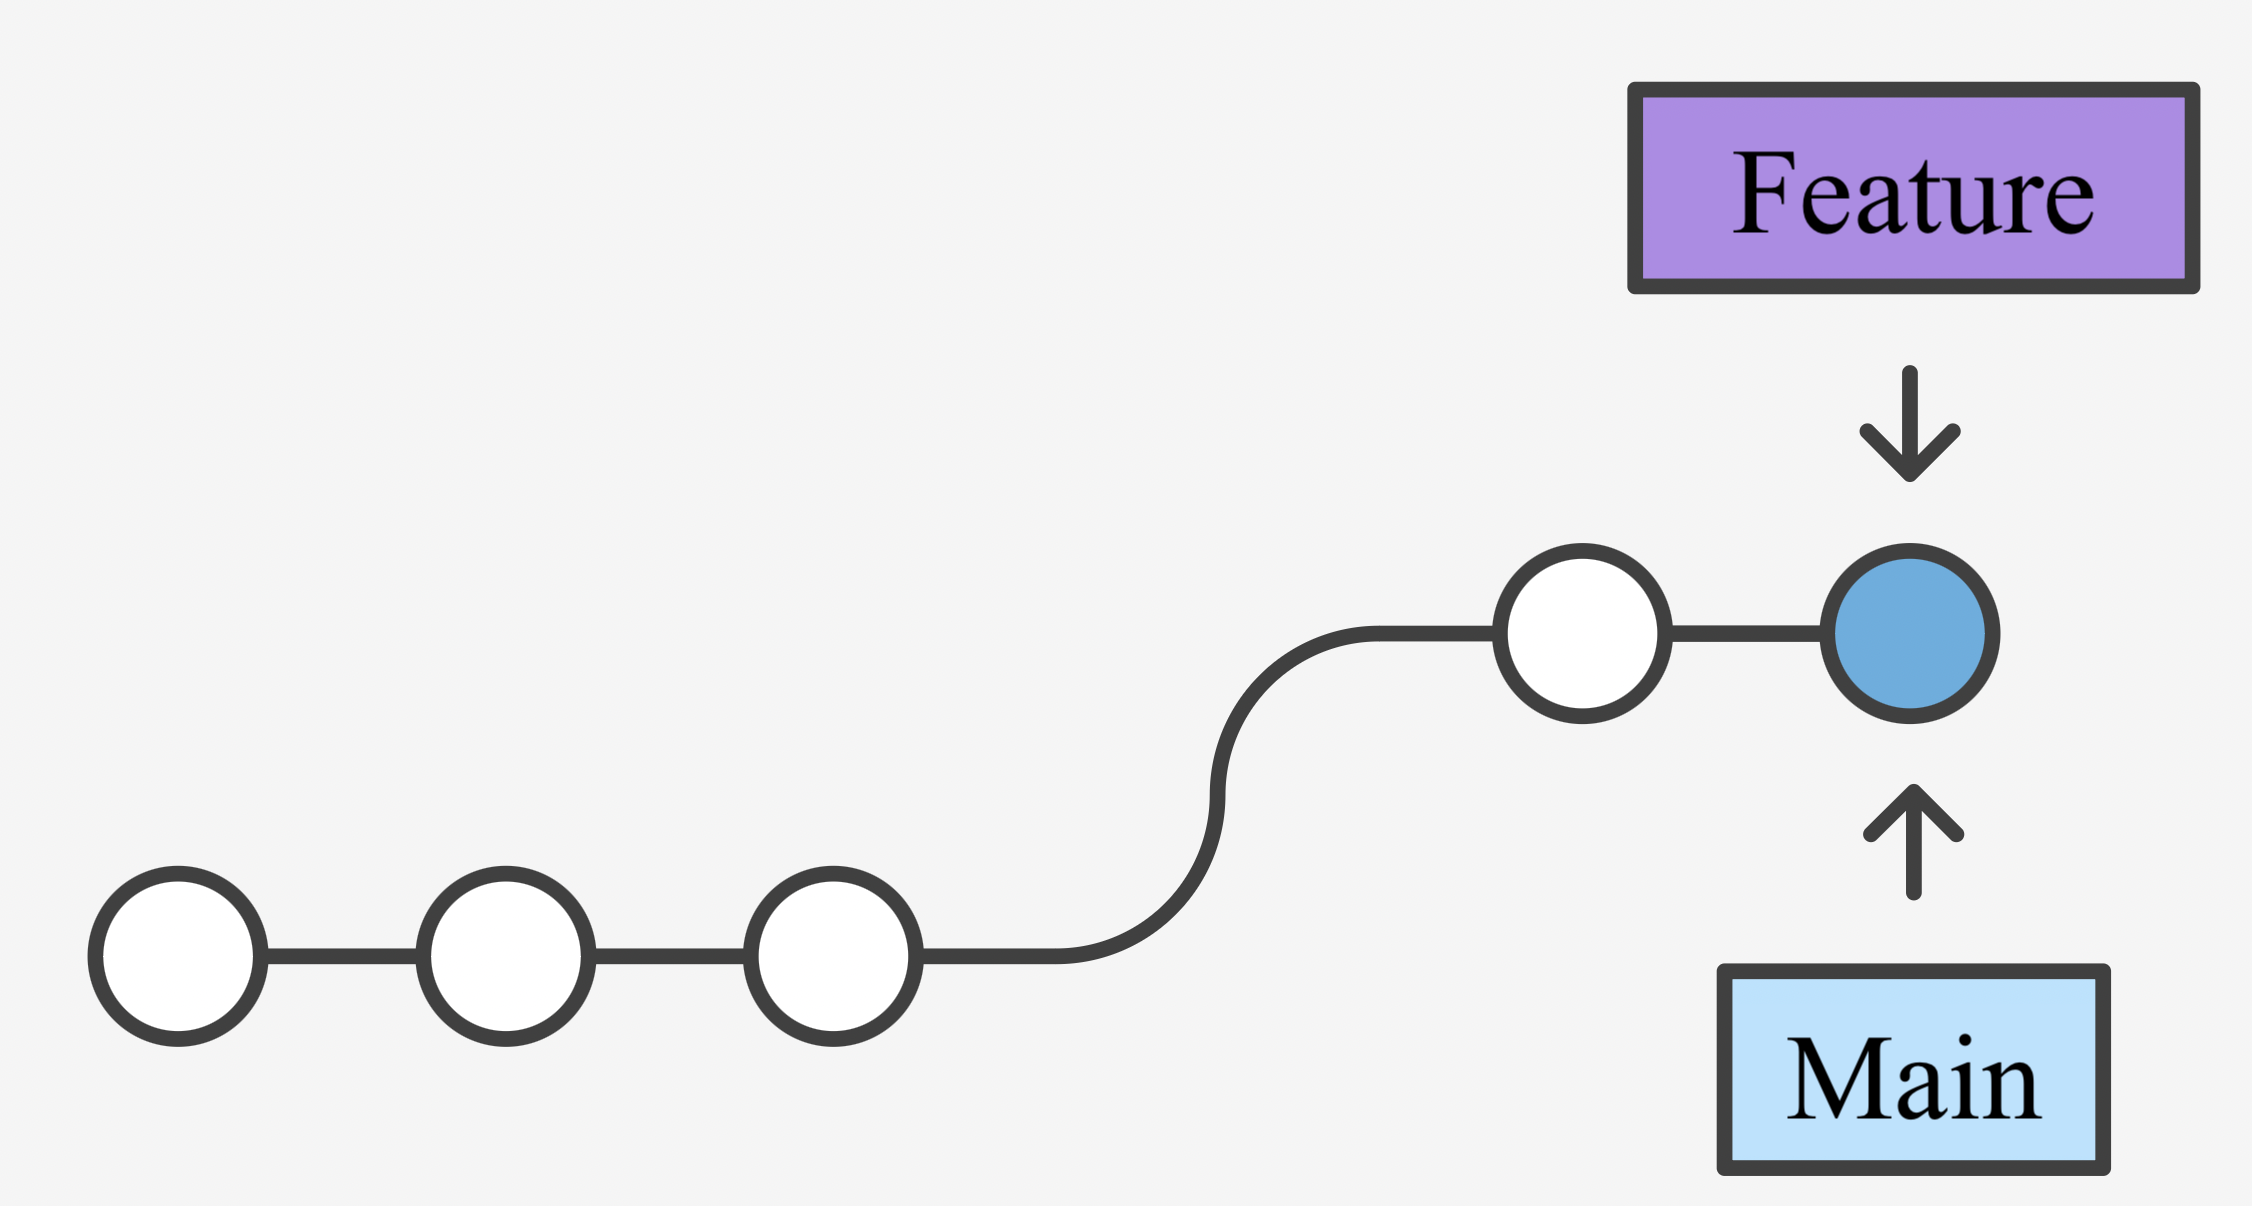
\includegraphics[width=\textwidth]{images/fast_forward_merge_after.png} 
				\captionsetup{justification=centering}
				\captionof{figure}{After a fast-forward merge. \href{https://www.atlassian.com/git/tutorials/using-branches/git-merge}{ \faLink{}  Source}}
			\end{minipage}
			
			
			
		\end{minipage}
	};
	\node[fancytitle, right=10pt, fill=outlinecolor, text=background, draw=outlinecolor, rounded corners] at (box.north west) {Branches};
\end{tikzpicture}